% CAPÍTULO 4 ESTADO DEL ARTE


\chapter{Estado del Arte}
\label{cap:estadoarte}

En este capítulo se muestran las plataformas, metodologías y proyectos de investigación orientados a la recolección,
sistematización y análisis de datos en el contexto de la violencia de género y sus consecuencias. Su analisispermite identificar la
brecha tecnológica actual y fundamentar el carácter innovador de la arquitectura propuesta en este Trabajo Terminal.
 
\section{Sistemas de monitoreo de medios tradicionales}
\label{sec:ea_monitoreo_tradicional}

En el ámbito de la inteligencia de fuentes abiertas y el monitoreo comercial
existen plataformas con infraestructuras para la recolección de datos en tiempo real (por ejemplo
Google Alerts, Meltwater, Mention). Estas herramientas funcionan principalmente sobre arquitecturas
de agregación RSS y rastreadores web de propósito general.

La principal debilidad de estos sistemas viene de su dependencia de cadenas de texto
y expresiones regulares. Al carecer de capacidades de comprensión semántica, la búsqueda de
heurísticas combinadas como \textit{``feminicidio''} y \textit{``NNA''} o \textit{``menores''} produce un volumen
estadísticamente inmanejable de ruido informativo y falsos positivos. Esta limitación fue demostrada
el prototipo 1 que fue basado en 15 palabras clave  con vectorización TF-IDF
y agrupamiento K-Means y que registró una tasa de falsos positivos del \textbf{80\%}. El prototipo 2 que
basó su detector en 72 patrones regex distribuidos en tres categorías (40 de feminicidio, 15 de NNA
y 17 de exclusión) obtuvo una reducción de los falsos positivos a un \textbf{60\%} lo que
demostró el límite sintáctico del paradigma léxico. Estos sistemas son incapaces de distinguir sintácticamente
entre un reporte donde el agresor resultó ser menor de edad, una noticia puramente estadística o un
caso donde un menor quedó en orfandad como víctima indirecta, pues la co-ocurrencia de palabras no
implica la co-ocurrencia de los roles semánticos que esas palabras desempeñan en la oración. Esta
incapacidad de inferencia contextual hace que las herramientas tradicionales resulten operativamente
ineficaces para el dominio específico de este proyecto.

\section{NLP aplicado a la detección de violencia de género}
\label{sec:ea_nlp_violencia}

Desde la perspectiva académica la intersección entre el procesamiento de lenguaje natural (PLN) y
la sociología forense ha ganado interés en los ultimos años. La literatura documenta la
transición de modelos de aprendizaje automático superficial (como \textit{Support Vector Machines}
o \textit{Random Forests}) hacia arquitecturas de aprendizaje profundo para la
clasificación de discursos de odio, misoginia en redes sociales y categorización automática de reportes
policiales por violencia doméstica.

Recientemente se han implementado modelos basados en Transformers (como RoBERTa y BERT) para extraer
relaciones de causalidad en narrativas de violencia armada y feminicidios documentados en la prensa.
Sin embargo al realizar una revisión bibliográfica minuciosa se nota una carencia de investigación
computacional enfocada en las víctimas indirectas. La inmensa mayoría de los clasificadores binarios
se detienen en la categorización del evento violento (feminicidio vs. homicidio culposo) lo que omite
por completo la extracción de entidades relacionadas con los NNA afectados.

\section{Herramientas y esfuerzos existentes en México}
\label{sec:ea_esfuerzos_mexico}

En México ante la insuficiencia de datos gubernamentales en tiempo real la sociedad civil ha
asumido tareas de investigación en la documentación de la violencia feminicida, desarrollando
iniciativas fundamentales que si bien son invaluables, presentan limitaciones de escalabilidad
computacional.

\subsection{Red por los Derechos de la Infancia en México (REDIM)}
La REDIM es la entidad sociopolítica más prominente en la articulación de datos macroeconómicos y
demográficos sobre la niñez mexicana. Sus informes sobre las infancias vulneradas son
fundamentales para el diseño de políticas públicas \cite{redim2023informe}. No obstante, a nivel
metodológico la organización depende fuertemente de la agregación estadística derivada de
solicitudes formales de transparencia, bases de datos gubernamentales que frecuentemente estan
desfasadas o censos . En consecuencia la REDIM carece de una plataforma tecnológica de
trazabilidad que opere mediante recolección automatizada de medios de comunicación masiva.

\subsection{El Mapa de los Feminicidios en México}
El proyecto cartográfico desarrollado por la investigadora María Salguero constituye un esfuerzo
pionero e históricamente vital para la visibilización geográfica de la crisis \cite{salguero2019mapa}.
El sistema geolocaliza y documenta variables sociodemográficas complejas. Sin embargo su principal
cuello de botella es arquitectónico en cuanto a que la recolección, lectura, extracción de características y
captura en base de datos de cada caso reportado en prensa que debido a la falta de una metodología bien definida
obedece a un flujo de trabajo manual y artesanal. Esta dependencia absoluta de la intervención humana
imposibilita el análisis retrospectivo masivo de fuentes hemerográficas a velocidad
computacional.

\subsection{Fundación Futuro con Derechos}
Organizaciones civiles dedicadas a la intervención directa como la Fundación Futuro con
Derechos, ilustran el problema operativo mas claramente. En su intento por identificar casos
emergentes de orfandad para ofrecer resguardo institucional o asesoría legal, el personal de
estas organizaciones invierte rutinariamente muchas horas semanales realizando búsquedas
manuales en portales de noticias. Este proceso no es escalable, propenso a sesgos de fatiga y
económicamente insostenible para asociaciones sin fines de lucro.

\section{Análisis comparativo y brecha identificada}
\label{sec:ea_brecha}

El análisis del estado actual del arte revela una brecha tecnológica bajo los paradigmas actuales
que es la desconexión entre la recolección masiva de datos no estructurados y la
comprensión semántica profunda de las víctimas indirectas. Las herramientas comerciales recolectan sin
comprender, mientras que los esfuerzos civiles comprenden profundamente pero no logran recolectar ni
escalar la información de forma automatizada.

La aportación fundamental de este Trabajo Terminal radica precisamente en la solución de esta problemática.
El sistema propuesto no es un simple buscador de palabras clave ni un mapa de captura manual. Su propuesta
radica en la orquestación integral de un flujo de trabajo automatizado que minimiza la
intervención humana en las etapas de descubrimiento y filtrado de información.

\section{Técnicas de extracción de datos}
\label{sec:ea_tecnicas_extraccion}

La recolección de datos periodísticos en fuentes abiertas es un problema
técnico pues los medios de comunicación digitales han colocado capas de
defensa cuyo objetivo es la protección contra el scraping masivo. La selección de la técnica
de extracción adecuada determina directamente la cobertura alcanzable del sistema,
tasa de éxito y su consumo de recursos computacionales. En la literatura de
recuperación de información se identifican
tres vertientes metodológicas principales y que se evaluaron
en función de su efectividad y eficiencia para la recolección de datos
periodísticos en México. 

\subsection{Extracción Estática (HTML Parsing con BeautifulSoup)}
\label{subsec:ea_beautifulsoup}

La aproximación más básica al \textit{web scraping} consiste en emitir una
petición HTTP directa al servidor objetivo y analizar sintácticamente el documento
HTML retornado mediante librerías de \textit{parsing} como \texttt{BeautifulSoup}
(Python) o \texttt{Cheerio} (Node.js). Esta técnica  fundamentada en la similitud
estructural del DOM y un árbol XML, permite la extracción
puntual de elementos textuales mediante selectores CSS o XPath.

Su principal limitación estructural es doble. En primer lugar los portales
informativos modernos construidos sobre \textit{frameworks} reactivos (React,
Vue, Angular) generan el DOM de forma dinámica en el cliente mediante JavaScript 
cosa que provoca que el HTML servido por el servidor carezca del contenido visible pues
solo existe tras la ejecución de decenas de \textit{bundles} de JavaScript 
\cite{wu2022dynamic}.
En segundo lugar los \textit{Web Application Firewalls} (WAF) de grado empresarial
(como Cloudflare, Akamai y PerimeterX) detectan las sesiones de
scraping estático mediante \textbf{TLS/JA3 fingerprinting} comparando el hash
criptográfico del saludo TLS (que identifica la librería SSL del cliente, por ejemplo
\texttt{Python/requests}) contra el User-Agent declarado.
Esta diferencia entre ambos activa el bloqueo con código \texttt{HTTP 403 Forbidden},
independientemente de los parámetros declarados por el scraper.

Esta fue la causa principal del fracaso del prototipo inicial durante el TT1, donde
el 100\% de los intentos de extracción directa sobre portales nacionales de alto
tráfico (La Jornada, El Universal, Milenio) resultaron en bloqueos sistemáticos y 
sin éxito.

\subsection{Automatización de navegador (Selenium / Playwright)}
\label{subsec:ea_selenium}

Para superar la barrera de los sitios con renderizado dinámico, la alternativa más
empleada en la investigación es la automatización de navegadores reales mediante
herramientas como \texttt{Selenium WebDriver} o \texttt{Playwright}
\cite{leotta2018web}. Estos \textit{frameworks} controlan una instancia
de Chrome o Firefox, ejecutando JavaScript en el entorno real del navegador y
resolviendo los desafíos JavaScript de Cloudflare de forma transparente.

Sin embargo esta aproximación manejaba costos operativos que resultan poco viables para
el dominio de este proyecto.

\begin{itemize}
    \item \textbf{Consumo de recursos:} Cada instancia del navegador requiere
          aproximadamente 150-300 MB de RAM y entre 5-15 segundos para cargar
          una página completa. Con un corpus objetivo de 45 fuentes y ciclos de
          recolección cada periodicas el costo computacional acumulado superaba los
          recursos disponibles en computadoras de desarrollo con recursos limitados.

    \item \textbf{Fragilidad estructural:} Los selectores CSS y XPath codificados
          en los scripts de extracción son altamente frágiles ante
          actualizaciones del diseño del portal. En entornos de despliegue continuo
          los identificadores de elementos HTML pueden cambiar en cualquier
          ciclo de publicación lo que requiere mantenimiento constante.

    \item \textbf{Detección avanzada por comportamiento:} Los sistemas anti-bot de
          última generación (DataDome, Kasada) analizan patrones de interacción
          (movimientos de ratón, secuencias de clicks, tiempos entre eventos) que
          los navegadores sin instrumentación adicional no logran reproducir
          fielmente por lo que el resultaba igualmente en bloqueos.
\end{itemize}

Por estas razones Selenium y Playwright se evaluaron pero descartaron como
técnica primaria de recolección y quedando a reserva de ser utilizados
como último recurso para fuentes sin alternativa RSS disponible.

\subsection{Agregación estructurada (RSS/Atom) y stealth sessions}
\label{subsec:ea_rss_stealth}

El protocolo \textbf{RSS} (\textit{Really Simple Syndication}) y su sucesor
\textbf{Atom} representan la alternativa técnicamente superior para la
monitorización continua de medios periodísticos. Ambos estándares definen
un formato XML normalizado que los medios publican voluntariamente para sindicar
su contenido y eliminando asi la necesidad de parsear HTML no estructurado
\cite{hammersley2005developing}. Las ventajas operativas son significativas.

\begin{enumerate}
    \item \textbf{Eficiencia de banda ancha:} Un feed RSS típico contiene los
          titulares, resúmenes y metadatos (fecha, autor, categoría) de los
          últimos 20-50 artículos en un documento XML de \textless~50 KB,
          frente a los 500 KB-2 MB de una página HTML completa con recursos
          estáticos. La reducción en consumo de ancho de banda es considerable.

    \item \textbf{Estabilidad del formato:} El esquema XML de RSS 2.0 es un
          estándar fijo pues los feeds no cambian su estructura ante
          actualizaciones de diseño del portal eliminando asi la fragilidad de
          los selectores CSS.

    \item \textbf{Ausencia de barreras WAF:} Los endpoints RSS son recursos
          públicos destinados explícitamente a la recolección automatizada por lo que los
          WAF no aplican \textit{fingerprinting} TLS sobre ellos. El sistema
          los consume con su identificador de bot legítimo sin técnicas de evasión.
\end{enumerate}

Para las fuentes que no exponen feeds RSS (que era cercano al 40\% del corpus
objetivo) en TT II se implementó \texttt{StealthSession} que es una capa de sesión
HTTP que resuelve los tres problemas identificados en el scraping estático:
(a)~emulación de fingerprint TLS mediante \texttt{cloudscraper},
(b)~delays con distribución log-normal que imitan patrones de lectura humana
y (c)~un \textit{Circuit Breaker} por dominio que evita el bloqueo permanente
de IP tras fallos consecutivos. Esta arquitectura híbrida RSS+StealthSession
logra cubrir la totalidad del corpus objetivo con una tasa de éxito de recolección
superior al 80\% en condiciones de producción.

\subsection{Tabla comparativa de técnicas de extracción}
\label{subsec:ea_tabla_scraping}

La Tabla~\ref{tab:comparativa_scraping} sintetiza la evaluación cuantitativa y
cualitativa de las tres vertientes analizadas en función de los criterios
operativos críticos para el sistema desarrollado.

\vspace{0.5cm}
\begin{table}[htbp]
\centering
\caption{Comparativa de técnicas de extracción}
\label{tab:comparativa_scraping}
\begin{tabular}{|p{2.8cm}|p{2.8cm}|p{2.8cm}|p{3.2cm}|}
\hline
\textbf{Criterio} &
\textbf{HTML Estático} \newline (BeautifulSoup) &
\textbf{Navegador} \newline (Selenium) &
\textbf{RSS + StealthSession} \newline (Implementado) \\
\hline
\textbf{Velocidad de extracción} &
Alta (0.5-2 seg por petición) &
Baja (5-15 seg por petición) &
Muy alta (0.3-1 seg por petición RSS, 8-20 seg por petición stealth) \\
\hline
\textbf{Resiliencia ante WAF} &
Muy baja (bloqueado por JA3 fingerprint) &
Media (bloqueado por análisis de comportamiento) &
Alta (RSS exento, stealth emula fingerprint TLS real) \\
\hline
\textbf{Estructura de datos} &
No estructurada (HTML variable) &
No estructurada (DOM dinámico) &
Estructurada (XML/RSS normalizado) \\
\hline
\textbf{Consumo de RAM} &
Bajo (5 MB por petición) &
Muy alto (150-300 MB por instancia) &
Bajo (3 MB por petición RSS) \\
\hline
\textbf{Mantenimiento} &
Alto (selectores CSS frágiles) &
Muy alto (selectores + actualizaciones del navegador) &
Bajo (esquema RSS inmutable) \\
\hline
\textbf{Cobertura de fuentes} &
Alta (cualquier sitio) &
Alta (cualquier sitio) &
Media (solo fuentes con RSS o stealth-compatible) \\
\hline
\textbf{Resultado en TT1/TT2} &
\textit{Descartado} (0\% éxito) &
\textit{Descartado} (recursos limitados) &
\textbf{Seleccionado} (mas del 80\% de éxito) \\
\hline
\end{tabular}
\end{table}
\vspace{0.4cm}

%----------------------------------------------------------------------------------------
\section{Evolución del almacenamiento}
\label{sec:ea_almacenamiento}
%----------------------------------------------------------------------------------------

La decisión de migrar el sistema de persistencia fue uno de los puntos mas
relevantes en  TT II. El análisis del estado del arte en almacenamiento de datos
para sistemas de recolección de noticias revela una clara división paradigmática:
los archivos planos (CSV/JSON) y los gestores de bases de datos relacionales (RDBMS).

\subsection{Archivos planos (CSV)}
\label{subsec:ea_csv}

Los archivos en formato \textit{Comma-Separated Values} (CSV) constituyeron el
mecanismo de persistencia del TT I por razones practicas como instalación cero,
compatibilidad universal con Pandas y ausencia de dependencias de infraestructura.
En el contexto de un prototipo inicial con corpus de aproximadamente 281
registros, estas ventajas superaban sus limitaciones.

La cuestion es que el análisis de capacidad hacia el final del TT I evidenció tres
limitaciones estructurales que establecen el techo operativo del paradigma CSV.

\begin{itemize}
    \item \textbf{Complejidad de consulta $O(n)$:} Cualquier operación de filtrado
          (ej.\ ``todas las noticias de Alta relevancia en Veracruz desde enero'')
          requiere cargar el archivo completo en memoria RAM y aplicar filtros en
          Python con complejidad lineal sobre el corpus. Proyectado a escala
          nacional con miles de noticias mensuales  esta operación agota los
          recursos de un servidor de desarrollo en segundos.

    \item \textbf{Ausencia de integridad referencial:} El esquema plano impide
          establecer relaciones entre entidades (noticias, fuentes, clusters,
          detecciones) con garantías de consistencia. Una noticia eliminada puede
          dejar registros de detección huérfanos sin mecanismo alguno de detección.

    \item \textbf{Concurrencia insegura:} La escritura simultánea desde el flujo
          analítico y la lectura desde el dashboard Flask sobre el mismo archivo CSV
          generan condiciones de carrera que pueden corromper los datos.
\end{itemize}

\subsection{PostgreSQL}
\label{subsec:ea_postgresql}

PostgreSQL fue seleccionado como motor de base de datos del TT2 II frente a
alternativas como MySQL, SQLite y bases de datos NoSQL (MongoDB, Elasticsearch)
por un conjunto de características técnicas específicamente necesarias para el
dominio del sistema e implementadas en \texttt{src/database/models\_noticias.py}.

\textbf{Modelo ACID y concurrencia segura.}
PostgreSQL implementa el estándar \textit{Atomicity, Consistency, Isolation,
Durability} (ACID) con el protocolo de control de concurrencia multiversión (MVCC),
que permite que múltiples lectores y un escritor operen simultáneamente sobre las
mismas tablas sin bloqueos ni corrupción de datos. Esta propiedad es imprescindible
en el sistema dado que el flujo analítico y el dashboard Flask ejecutan
transacciones concurrentes sobre la tabla \texttt{noticias}.

\textbf{Integridad referencial con \texttt{FOREIGN KEY}.}
El esquema relacional implementado en \texttt{models\_noticias.py} define cuatro
tablas con relaciones explícitas:

La restricción \texttt{ondelete="CASCADE"} garantiza que la eliminación de una
noticia propague automáticamente la eliminación de sus detecciones y entidades
asociadas lo que mantiene la integridad referencial sin lógica adicional en la
aplicación.

\textbf{Full-Text Search nativo con índices GIN.}
La característica más determinante para la selección de PostgreSQL frente a
MySQL o SQLite es su soporte nativo de búsqueda de texto completo (FTS) en
español. PostgreSQL implementa FTS mediante el tipo de dato \texttt{tsvector},
que almacena un vector léxico preprocesado (con \textit{stemming}, eliminación de
\textit{stop words} y normalización de acentos) del texto de cada documento.
Los índices de tipo \textbf{GIN} (\textit{Generalized Inverted Index}) sobre columnas
\texttt{tsvector} permiten resolver consultas FTS complejas en $O(\log n)$ mediante
una búsqueda de intersección de listas de postings invertidas en lugar del escaneo
lineal $O(n)$ que impone cualquier búsqueda \texttt{LIKE '\%...\%'} en MySQL o SQLite.

\textbf{Contraste con alternativas NoSQL.}
Sistemas como MongoDB o Elasticsearch podrían ofrecer capacidades de búsqueda
de texto completo pero a costa de las garantías ACID y la integridad referencial.
En un sistema de monitoreo de derechos humanos donde la consistencia de los datos
es un requisito ético y operativo no negociable, la ausencia de transacciones
ACID en bases de datos NoSQL representa un riesgo. Elasticsearch
aunque ofrece FTS de calidad comparable requiere un stack de infraestructura
adicional (JVM, configuración de cluster) incompatible con las restricciones
de recursos del entorno.

\begin{figure}[htbp]
\centering
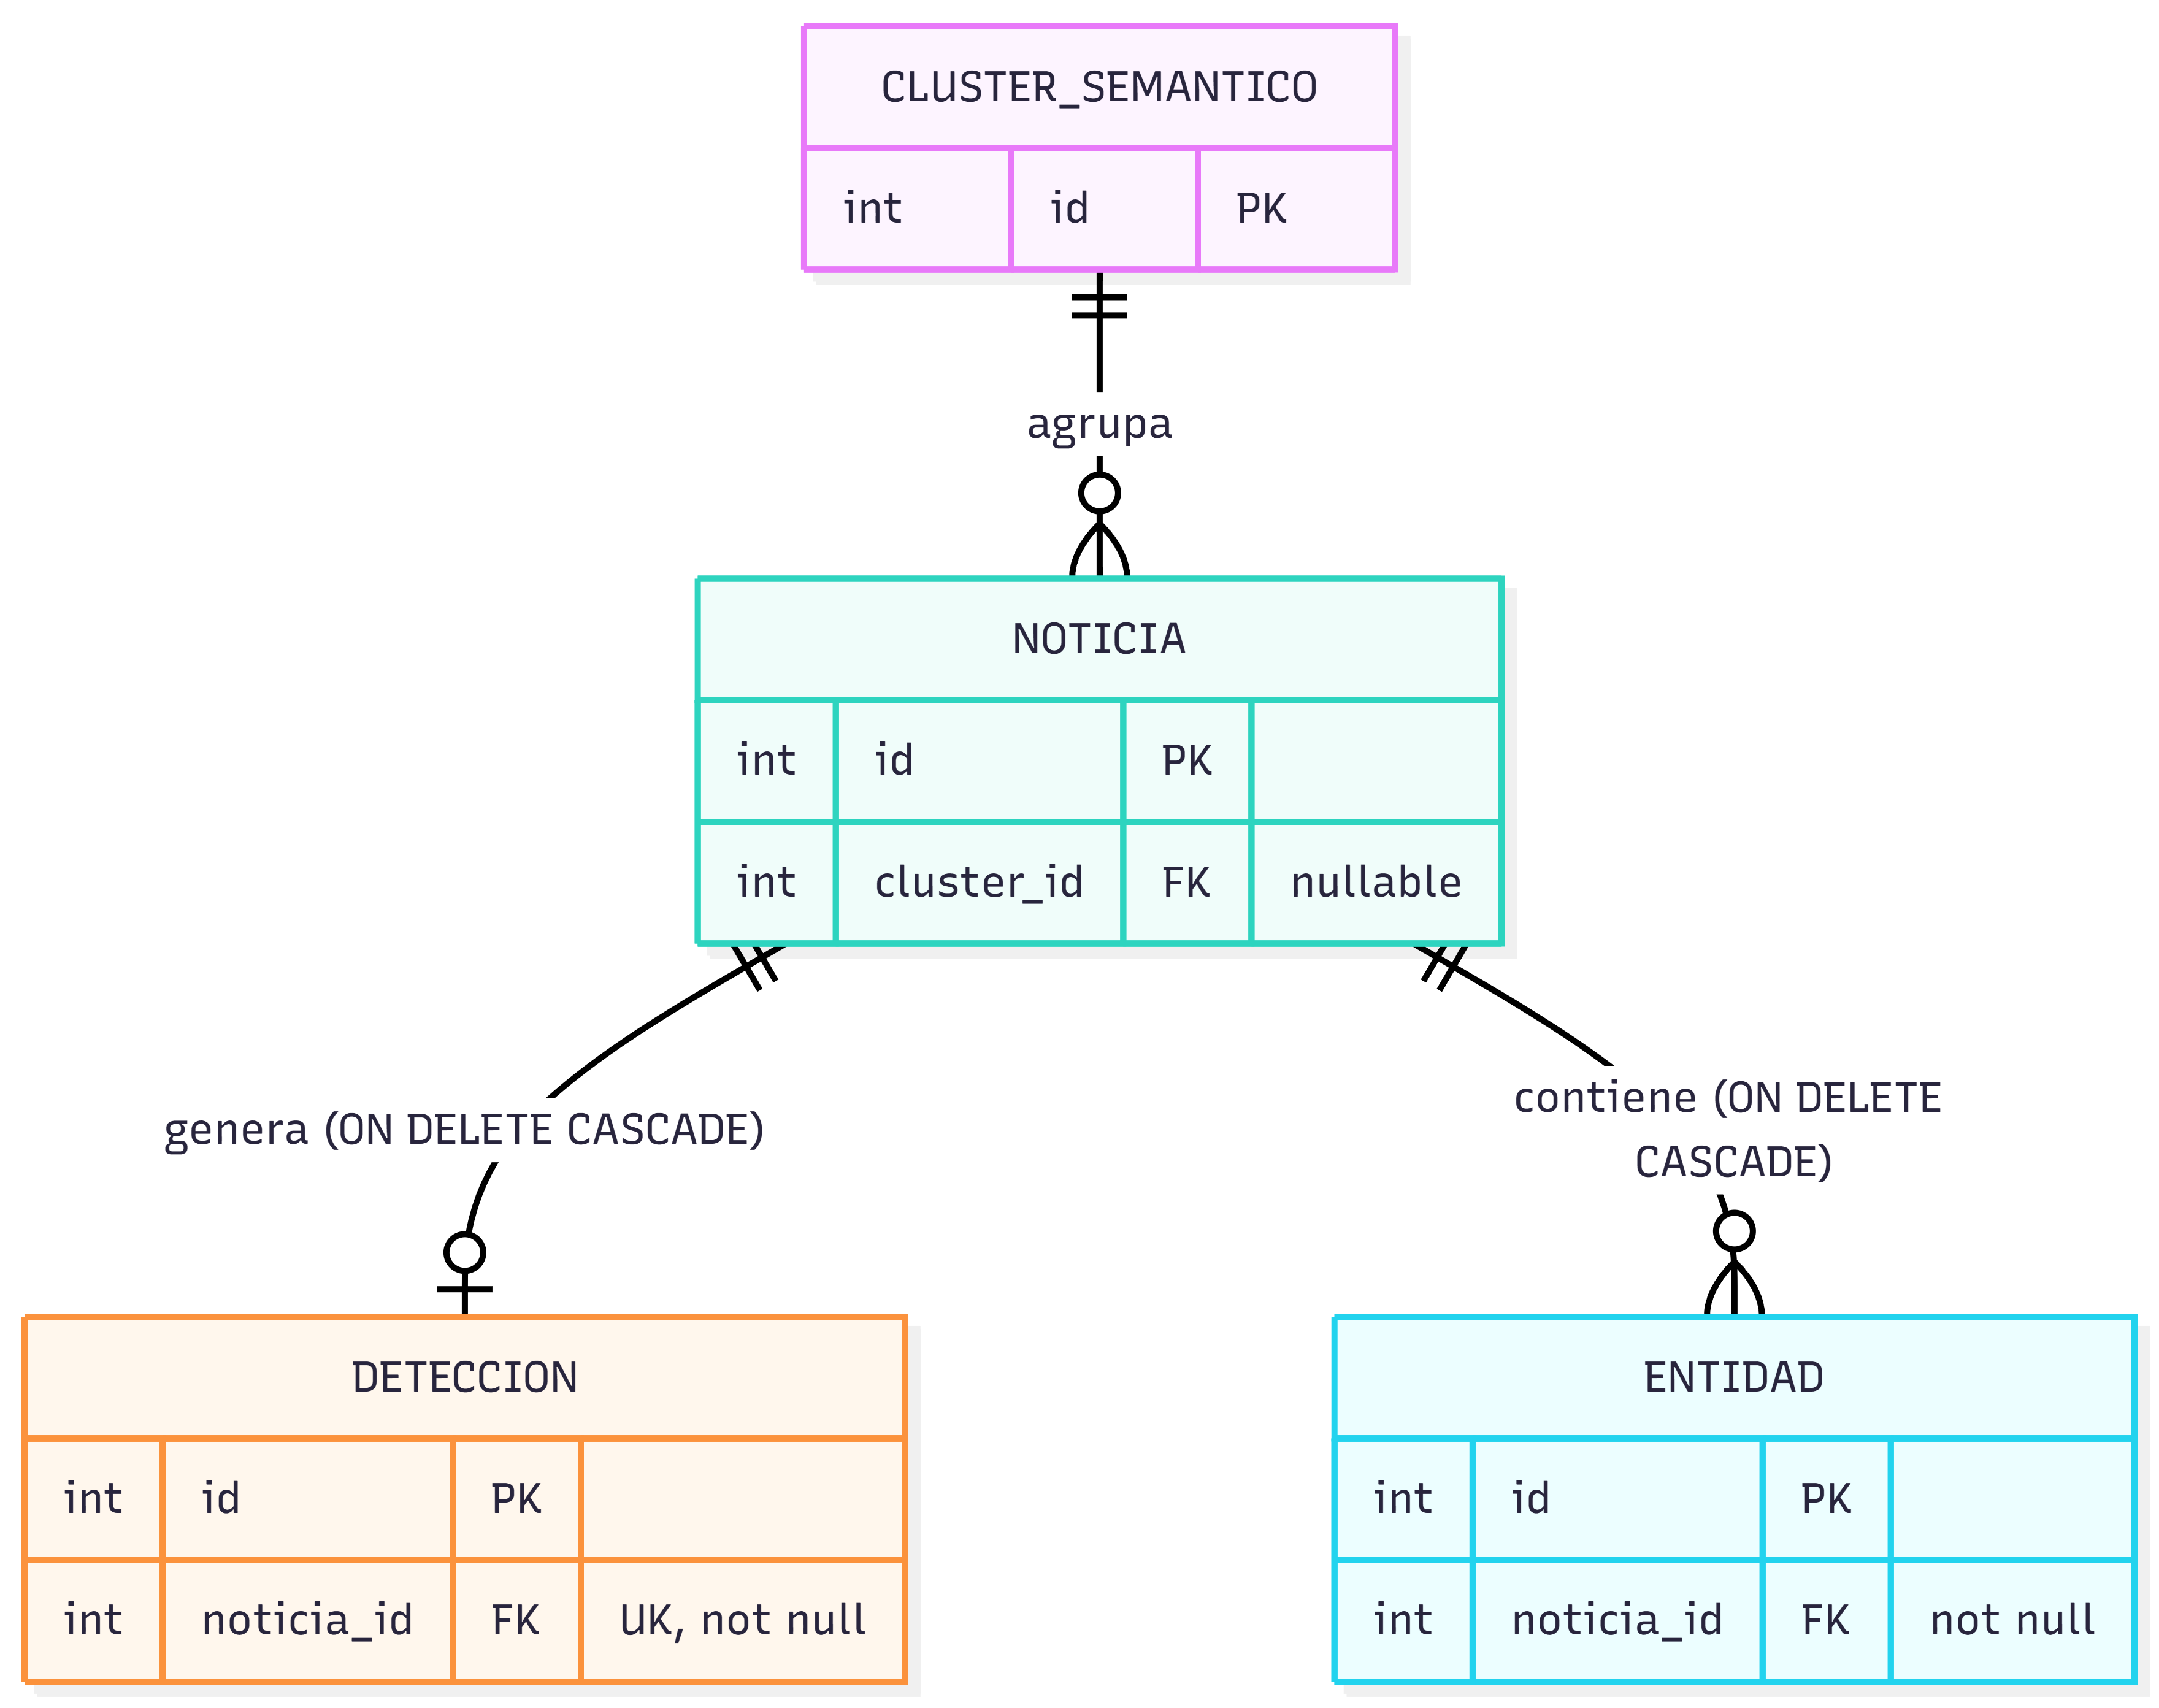
\includegraphics[width=\textwidth]{images/bdarte.png}
\caption{Esquema relacional}
\label{fig:esquema_db}
\end{figure}

\clearpage

\section{Evolución de los modelos de representación lingüística para NLP}
\label{sec:ea_modelos_nlp}


La selección del motor de clasificación semántica fue una de las decisiones más
importantes en la arquitectura del TT II. La evolución histórica del campo del
Procesamiento de Lenguaje Natural (PLN) describe una trayectoria en la que cada
generación de modelos supera las limitaciones fundamentales de la anterior, no solo
en precisión medida sino en la profundidad del fenómeno lingüístico que es capaz de
capturar. Esta sección examina las tres generaciones de representaciones lingüísticas
evaluadas durante el diseño del sistema.

\subsection{Word2Vec y GloVe}
\label{subsec:ea_word2vec}

Los modelos de incrustación de palabras (\textit{word embeddings}) de primera
generación Word2Vec \cite{mikolov2013word2vec} y GloVe \cite{pennington2014glove}
representaron un salto cualitativo respecto al paradigma de vectores dispersos
de TF-IDF, al proyectar el vocabulario en un espacio vectorial denso de dimensión
reducida (100-300 dimensiones) donde la proximidad geométrica captura similitud
semántica.

No obstante ambos modelos comparten una limitación estructural determinante pues es
la asignación de un único vector por palabra, independientemente del contexto.
El token ``menor'' recibe la misma representación vectorial en
``un menor infractor detenido'' que en
``sus menores hijos quedaron huérfanos''. Esta limitación no resuelta
es exactamente el mecanismo de falla que generó la mayoria de falsos positivos
en el motor heurístico del TT I donde la co-ocurrencia de tokens de dominio sin
discernimiento de rol semántico era el método de clasificación. 

\subsection{LSTM y GRU} 
\label{subsec:ea_lstm}

Las redes de memoria a largo y corto plazo (LSTM) \cite{hochreiter1997lstm}
introdujeron la modelización del contexto \textit{secuencial} que es la representación
de un token que se calcula en función de todos los tokens precedentes. No obstante
presentan tres limitaciones técnicas inadecuadas para el dominio de este sistema.

\begin{enumerate}
    \item \textbf{Contexto unidireccional.} El modelo no puede leer ``hacia adelante''
          para resolver ambigüedades de rol semántico. En \textit{``la mujer asesinada
          dejó tres hijos menores''}, ``menores'' solo recibe contexto izquierdo,
          sin considerar que ``resguardo del DIF'' (derecha) confirma el rol
          de víctima indirecta.

    \item \textbf{Degradación del gradiente a largo alcance.} Las dependencias
          semánticas que abarcan más de 40-50 tokens presentan degradación en la
          retropropagación lo que limita la correlación sujeto-predicado en oraciones
          compuestas.

    \item \textbf{Paralelización imposible.} La naturaleza secuencial impide el
          procesamiento paralelo en GPU lo que significa que el token $t$ no puede ser procesado
          hasta que el estado oculto del token $t-1$ esté disponible.
\end{enumerate}

\subsection{BERT}
\label{subsec:ea_transformer}

La arquitectura \textit{Transformer} \cite{vaswani2017attention} resuelve
simultáneamente las tres limitaciones anteriores mediante el mecanismo de
\textbf{autoatención multi-cabeza} pues para cada token de la secuencia se calcula
un vector de atención ponderada sobre \textit{todos} los demás tokens de forma
simultánea. BERT \cite{devlin2019bert} extiende este paradigma mediante el
preentrenamiento bidireccional con Modelado de Lenguaje Enmascarado (MLM),
forzando representaciones que consideran simultáneamente el contexto izquierdo
y derecho de cada token.

Para el dominio de este proyecto, la bidireccionalidad es la propiedad
técnicamente decisiva pues la representación de ``menor'' en
\textit{``sus hijos menores quedaron en resguardo del DIF''} se calcula
considerando tanto ``hijos'' (izquierda) como ``resguardo del DIF'' (derecha),
produciendo un embedding que captura inequívocamente el rol de víctima indirecta.
Esta es la capacidad que el motor RegEx del TT I no pudo aproximar.

\subsection{Justificación de BETO frente a Modelos Multilingües (mBERT)}
\label{subsec:ea_beto_vs_mbert}

En el ecosistema de modelos preentrenados en español la alternativa más inmediata
a BETO es \textbf{mBERT} (\textit{multilingual BERT}) que es un modelo de Google entrenado
sobre Wikipedia en 104 idiomas pero que la cobertura multi-idioma introduce
un compromiso técnico significativo pues al distribuir la capacidad representacional de
sus 110 millones de parámetros entre 104 lenguas la calidad de representación del
español es inherentemente inferior a la de un modelo monolingüe del mismo tamaño.
Estudios de evaluación comparativa reportan que BETO supera a mBERT en un 3-8\%
de precición en tareas de clasificación de texto en español \cite{canete2020beto}.

\textbf{BETO} (\textit{dccuchile/bert-base-spanish-wwm-cased}) \cite{canete2020beto},
desarrollado por la Universidad de Chile se entrenó exclusivamente en español
a partir de Wikipedia en español ($\sim$3 GB, con 42 millones de oraciones), corpus
OPUS (OpenSubtitles, ParaCrawl, MultiUN) y fuentes de prensa latinoamericana.
La inclusión de este último componente es importante pues sesga
positivamente las representaciones hacia el vocabulario y estilo redaccional
de los medios de comunicación mexicanos lo que es exactamente el tipo de texto
que el sistema procesa. El entrenamiento con \textit{Whole Word Masking} (WWM)
garantiza además que los términos especializados de múltiples sub-tokens
(como \texttt{femi\#\#ni\#\#cid\#\#io}) se aprendan como unidades semánticas
coherentes.

La Tabla~\ref{tab:comparativa_modelos_nlp} presenta la evaluación comparativa
de los modelos considerados.

\vspace{0.5cm}
\begin{table}[htbp]
\centering
\caption{Comparativa de modelos de representación lingüística para clasificación semántica}
\label{tab:comparativa_modelos_nlp}
\begin{tabular}{|p{2.2cm}|p{3.0cm}|p{2.4cm}|p{2.4cm}|p{1.8cm}|}
\hline
\textbf{Modelo} &
\textbf{Comprensión contextual} &
\textbf{Idioma nativo} &
\textbf{Hardware requerido} &
\textbf{Resultado} \\
\hline
TF-IDF + RegEx (TT I) &
Ninguna (co-ocurrencia léxica) &
Ninguno (estadístico) &
CPU, menos de 1 GB RAM &
\textit{Descartado} (80\% FP en P1, 60\% en P2) \\
\hline
Word2Vec/GloVe &
Estática (sin contexto) &
Español limitado &
CPU, menos de 2 GB RAM &
\textit{Descartado} (ambigüedad léxica) \\
\hline
LSTM/GRU &
Secuencial unidireccional &
Requiere reentrenamiento &
GPU recomendada &
\textit{Descartado} (gradiente, velocidad) \\
\hline
mBERT &
Bidireccional (en 104 idiomas) &
Multilingüe (sesgo reducido en español) &
Alrededor de 8 GB RAM (CPU viable) &
\textit{Considerado} (superado por BETO en español) \\
\hline
\textbf{BETO} &
\textbf{Bidireccional plena} &
\textbf{Español monolingüe nativo} &
\textbf{Alrededor de 8 GB RAM (CPU viable)} &
\textbf{Seleccionado} \\
\hline
GPT-4/Claude &
LLM (máxima capacidad) &
Multilingüe alta calidad &
API externa sin GPU local &
\textit{Descartado} (soberanía) \\
\hline
\end{tabular}
\end{table}
\vspace{0.4cm}

\subsection{Zero-Shot y su transición a clasificación escalonada}
\label{subsec:ea_zeroshot_vs_finetune}

Durante el prototipo 3 se implementó la estrategia de clasificación \textit{Zero-Shot} basada en la
similitud coseno entre los embeddings \texttt{[CLS]} de BETO y descripciones de categorías en lenguaje
natural ("relevante" y "no relevante"). Las similitudes crudas resultaron muy cercanas
(diferencias de 0.02-0.05) por lo que se aplicó \textit{Temperature Scaling} con factor térmico 5
para amplificar la separación probabilística antes de Softmax. Pero en la evaluación sobre un
corpus de $\sim$800 noticias se pudo ver una vulnerabilidad crítica denominada \textbf{efecto
péndulo} en el que el modelo oscilaba entre dos estados no deseados pues en cada recolección
había un exceso masivo de falsos positivos o un exceso masivo de falsos negativos por lo que se
requeria una mejora en la estrategia de clasificación. Esta inestabilidad se veía reflejada en tres
escenarios.

\begin{enumerate}
    \item El post-filtro de validación semántica aplicaba reglas binarias absolutas que degradaban
          noticias genuinas cuya redacción no coincidía con las frases esperadas.
    \item El filtro léxico bloqueaba completamente noticias con contenido mixto (un hecho de
          violencia que también mencionaba una iniciativa de ley relacionada).
    \item El modo \textit{zero-shot} era incapaz de distinguir entre \textit{``mujer asesinada que
          deja hijos''} y \textit{``ley que protege a hijos de mujeres asesinadas''} porque
          ambas oraciones comparten el mismo campo semántico en el espacio de embeddings.
\end{enumerate}

El estado del arte en ajuste de modelos fundacionales estableció que para superar el solapamiento
semántico en dominios específicos, el \textbf{Fine-Tuning supervisado} es necesario
\cite{peters2019tune}. Para mitigar el desafío de la escasez inicial de datos el paradigma de
\textit{Active Learning} \cite{settles2009active} se posiciona como la solución óptima permitiendo
que el sistema solicite etiquetado humano exclusivamente sobre los verdaderos negativos.
En consecuencia en el prototipo 4 se implementó una \textbf{arquitectura de clasificación escalonada}
con cuatro capas autónomas que operan secuencialmente sobre un score acumulativo.

\begin{description}
    \item[\textbf{Capa 0 escudo léxico}] Filtro de rechazo temprano que descarta dominios completamente
    ajenos al feminicidio (deportes, economía, tecnología). Es la única capa que produce bloqueo absoluto
    (\texttt{score = 0.0}).

    \item[\textbf{Capa 1 escudo suave}] Los términos legislativos y estadísticos que en el
    prototipo anterior producían bloqueo absoluto fueron migrados a un conjunto de penalización
    aditiva $\delta = -0.35$. Una noticia genuina con score BETO de 0.72 que menciona
    ``según datos del REDIM'' obtiene score ajustado de 0.37, clasificando como ``Media''
    en lugar de excluirse. Si el score BETO es alto ($\geq 0.95$), la noticia sobrevive
    como ``Alta'' ($0.95 - 0.35 = 0.60$).

    \item[\textbf{Capa 2 Inferencia BETO}] Opera con prioridad estricta, el clasificador
    \textit{Finetuned} tiene precedencia sobre el modo \textit{Zero-Shot}, que se activa
    automáticamente cuando el modelo ajustado no está disponible.

    \item[\textbf{Capa 3 Post-filtro de Validación}] Inyecta bonificaciones al detectar
    evidencia explícita de orfandad real (patrones como \texttt{qued[oó] al cuidado},
    \texttt{menores? (bajo|en) resguardo}) y penalizaciones al detectar roles invertidos
    (menor como agresor). Esta capa nunca produce exclusiones absolutas para noticias
    clasificadas como ``Media''.
\end{description}

Este diseño neuro-simbólico, donde las reglas simbólicas modulan la salida del componente neuronal
mediante penalizaciones y bonificaciones aditivas en lugar de rechazos binarios absolutos,
eliminó el efecto péndulo y representa la contribución más relevante de TT II.

\subsection{Soberanía de datos y rechazo de APIs privativas}
\label{subsec:ea_soberania_datos}

La decisión de ejecutar BETO localmente mediante PyTorch en lugar de delegar
la inferencia a APIs privativas (GPT-4, Claude, Gemini), se fundamenta en tres
argumentos no negociables:

\begin{enumerate}
    \item \textbf{Privacidad de los datos.} El sistema procesa información sobre
          feminicidios y víctimas menores de edad. La transmisión de este contenido
          a servidores corporativos externos implica riesgos de privacidad
          incompatibles con la LGDNNA y el principio de minimización de datos
          de la LFPDPPP.

    \item \textbf{Costo operativo sostenible.} La inferencia de GPT-4 para
          600-1{,}000 documentos por ciclo costaría \$15-\$40~USD por ejecución,
          proyectando \$450-\$1{,}200 USD mensuales en ciclos de 6 horas. BETO
          en CPU tiene costo variable cero.

    \item \textbf{Reproducibilidad científica.} Los modelos propietarios modifican
          silenciosamente sus pesos entre versiones lo que imposibilita la reproducción
          exacta de los resultados reportados. BETO es un modelo de pesos abiertos
          cuya revisión exacta queda fijada en el registro del proyecto.
\end{enumerate}

\subsection{Investigación profunda bajo demanda}
\label{subsec:ea_deepinvestigator}

Una limitación crítica identificada al finalizar el TT I era que el flujo de clasificación producía
\textit{clasificaciones de relevancia} pero no extraía información estructurada sobre
los casos específicos como quién era la víctima directa, cuántos menores quedaron huérfanos,
quién estaba a cargo de ellos, entre otros. Esta carencia era especialmente clave
para el propósito central del sistema, pues la intervención de organizaciones civiles requiere
fichas de caso accionables, no puntuaciones de relevancia.

La alternativa obvia habría sido integrar la investigación profunda dentro del flujo
recolector-analítico automático pero la implementación hizo evidentes dos problemas
dentro de las restricciones operativas del proyecto.

\begin{enumerate}
    \item \textbf{Latencia no tolerable.} Cada investigación implica al menos dos llamadas a
          DuckDuckGo (búsqueda y extracción de contenido) y dos llamadas a la API de Gemini
          Flash (generación de query y síntesis del JSON final), lo que elevaba el tiempo
          de ejecución del flujo completo entre 45 y 90 minutos adicionales.
    \item \textbf{Costo de API desproporcionado.} La API de Google Gemini opera bajo cuotas
          en el plan gratuito y la investigación automática de todas las noticias ``Alta''
          saturaba la cuota en el primer tercio del corpus.
\end{enumerate}

La solución adoptada siguió el paradigma \textbf{reactivo e interactivo}, en el cual el módulo
\texttt{DeepInvestigator} (\texttt{src/analysis/investigator.py}) se convierte en una
herramienta que el analista activa manualmente desde el dashboard sobre una noticia
específica. Activado, ejecuta cuatro pasos secuenciales.

\begin{enumerate}
    \item \textbf{Generación de query (Gemini Flash).} Se genera una frase de búsqueda
          de alta especificidad (máximo 6 palabras) a partir del título y los primeros párrafos,
          incluyendo el nombre de la víctima y detalles únicos del caso.
    \item \textbf{Búsqueda en DuckDuckGo.} La query se envía tanto a la versión HTML como a la
          versión Lite de DuckDuckGo para maximizar la cobertura ante bloqueos intermitentes.
    \item \textbf{Scraping de contenido complementario.} \texttt{StealthSession} extrae el texto
          de cada URL retornada, filtrando ruido HTML, y concatena hasta 15{,}000~caracteres
          de contexto.
    \item \textbf{Síntesis estructurada (Gemini Flash).} El bloque de texto se envía a Gemini
          con un prompt de analista criminal especializado en derechos de la infancia. La respuesta
          es un JSON estricto con siete campos: \texttt{ubicacion}, \texttt{victimas},
          \texttt{ninos\_afectados}, \texttt{edades}, \texttt{situacion\_actual},
          \texttt{medios\_contacto} y \texttt{resumen}.
\end{enumerate}

El módulo también expone un segundo caso de uso que es la \textbf{identificación por enlace externo},
mediante el cual el analista proporciona directamente la URL de una noticia que el flujo automático no detectó,
y el sistema reutiliza el mismo flujo para incorporarla. Esta funcionalidad completa el ciclo de la plataforma
convirtiendo el sistema en una herramienta colaborativa donde el criterio experto del analista y la potencia del
asistente automatizado se complementan.

\clearpage
\section{Técnicas de agrupamiento}
\label{sec:ea_clustering}


El agrupamiento automático de documentos periodísticos constituye el mecanismo
que permite al sistema trascender la clasificación individual de noticias y obtener
una comprensión del \textit{paisaje informativo} del periodo analizado. En lugar de
clasificar cada noticia en aislamiento, el agrupamiento semántico revela qué noticias
relatan el mismo evento criminal desde múltiples medios, qué clústeres temáticos
dominan el corpus en un periodo dado y qué documentos son \textit{outliers} sin
coherencia temática con el resto. Esta perspectiva global es imposible mediante
clasificación individual y es una propiedad emergente del corpus completo.

\subsection{Métodos tradicionales}
\label{subsec:ea_kmeans}

El algoritmo K-Means \cite{lloyd1982least} es el método de agrupamiento por
centroides más extendido en la literatura de recuperación de información. Su
principio de funcionamiento consiste en minimizar la suma de distancias
euclidianas al cuadrado entre cada punto y el centroide de su clúster asignado,
mediante una convergencia iterativa de asignación y actualización de centroides.

La cuestion es que K-Means presenta dos limitaciones estructurales que lo hacian
inadecuado para el dominio de este sistema.

\begin{enumerate}
    \item \textbf{La maldición de la dimensionalidad.}
          Los embeddings de texto generados por BETO son vectores de 768 dimensiones.
          En espacios de alta dimensionalidad, la distancia euclidiana pierde su
          poder discriminatorio pues la diferencia entre la distancia al punto más
          cercano y al más lejano tiende a cero a medida que la dimensionalidad
          crece \cite{beyer1999nearest}. Este fenómeno hace que la noción de ``centroide
          más cercano'' sea geométricamente inestable, generando asignaciones de clúster
          arbitrarias. Esta fue la causa del bajo rendimiento de K-Means en TT I donde
          los clústeres resultantes no correspondían a grupos temáticamente coherentes sino
          a particiones geométricamente arbitrarias del espacio vectorial.

    \item \textbf{Requerimiento de \textit{k} fijo.} K-Means exige que el número
          de clústeres sea especificado. En un sistema donde el número de temas
          activos varía según los eventos noticiosos, esta rigidez es operativamente
          insostenible. Fijar $k=10$ en un periodo con solo 3 temas activos
          fragmenta artificialmente los clústeres reales y fijar $k=10$ en un
          periodo con 25 temas activos los colapsa en grupos heterogéneos.
\end{enumerate}

\subsection{DBSCAN}
\label{subsec:ea_dbscan}

El algoritmo DBSCAN \cite{ester1996dbscan} (\textit{Density-Based Spatial Clustering
of Applications with Noise}) supera la limitación del $k$ fijo al definir los
clústeres como regiones de alta densidad en el espacio métrico, separadas por
regiones de baja densidad. Los puntos que no pertenecen a ninguna región densa
son clasificados como \textit{ruido}, una propiedad fundamental para el dominio
de este proyecto donde las noticias genéricas no relacionadas con el tema central
deben ser identificadas y filtradas.

Sin embargo DBSCAN presenta una limitación crítica ante datos reales pues requiere
que la densidad de los clústeres sea \textit{uniforme}. El parámetro global de
radio de vecindad $\varepsilon$ define la densidad mínima de toda la solución, un
único valor de $\varepsilon$ no puede capturar simultáneamente clústeres de alta
densidad (eventos con cobertura mediática masiva de muchos medios) y clústeres de
baja densidad (casos locales cubiertos por pocos medios regionales). Esta limitación
genera segmentaciones inconsistentes en corpus periodísticos donde la cobertura
mediática de los eventos es inherentemente heterogénea.

\subsection{BERTopic}
\label{subsec:ea_bertopic}

BERTopic \cite{grootendorst2022bertopic} supera las limitaciones de K-Means y
DBSCAN mediante una arquitectura modular de cinco etapas que separa la
representación, la reducción de dimensionalidad, el clustering y la
representación de tópicos en componentes independientes y sustituibles. La
implementación en \texttt{src/analysis/bertopic\_clustering.py} instancia esta
arquitectura con parámetros calibrados específicamente para el corpus periodístico en
español.

\begin{figure}[H]
    \centering
    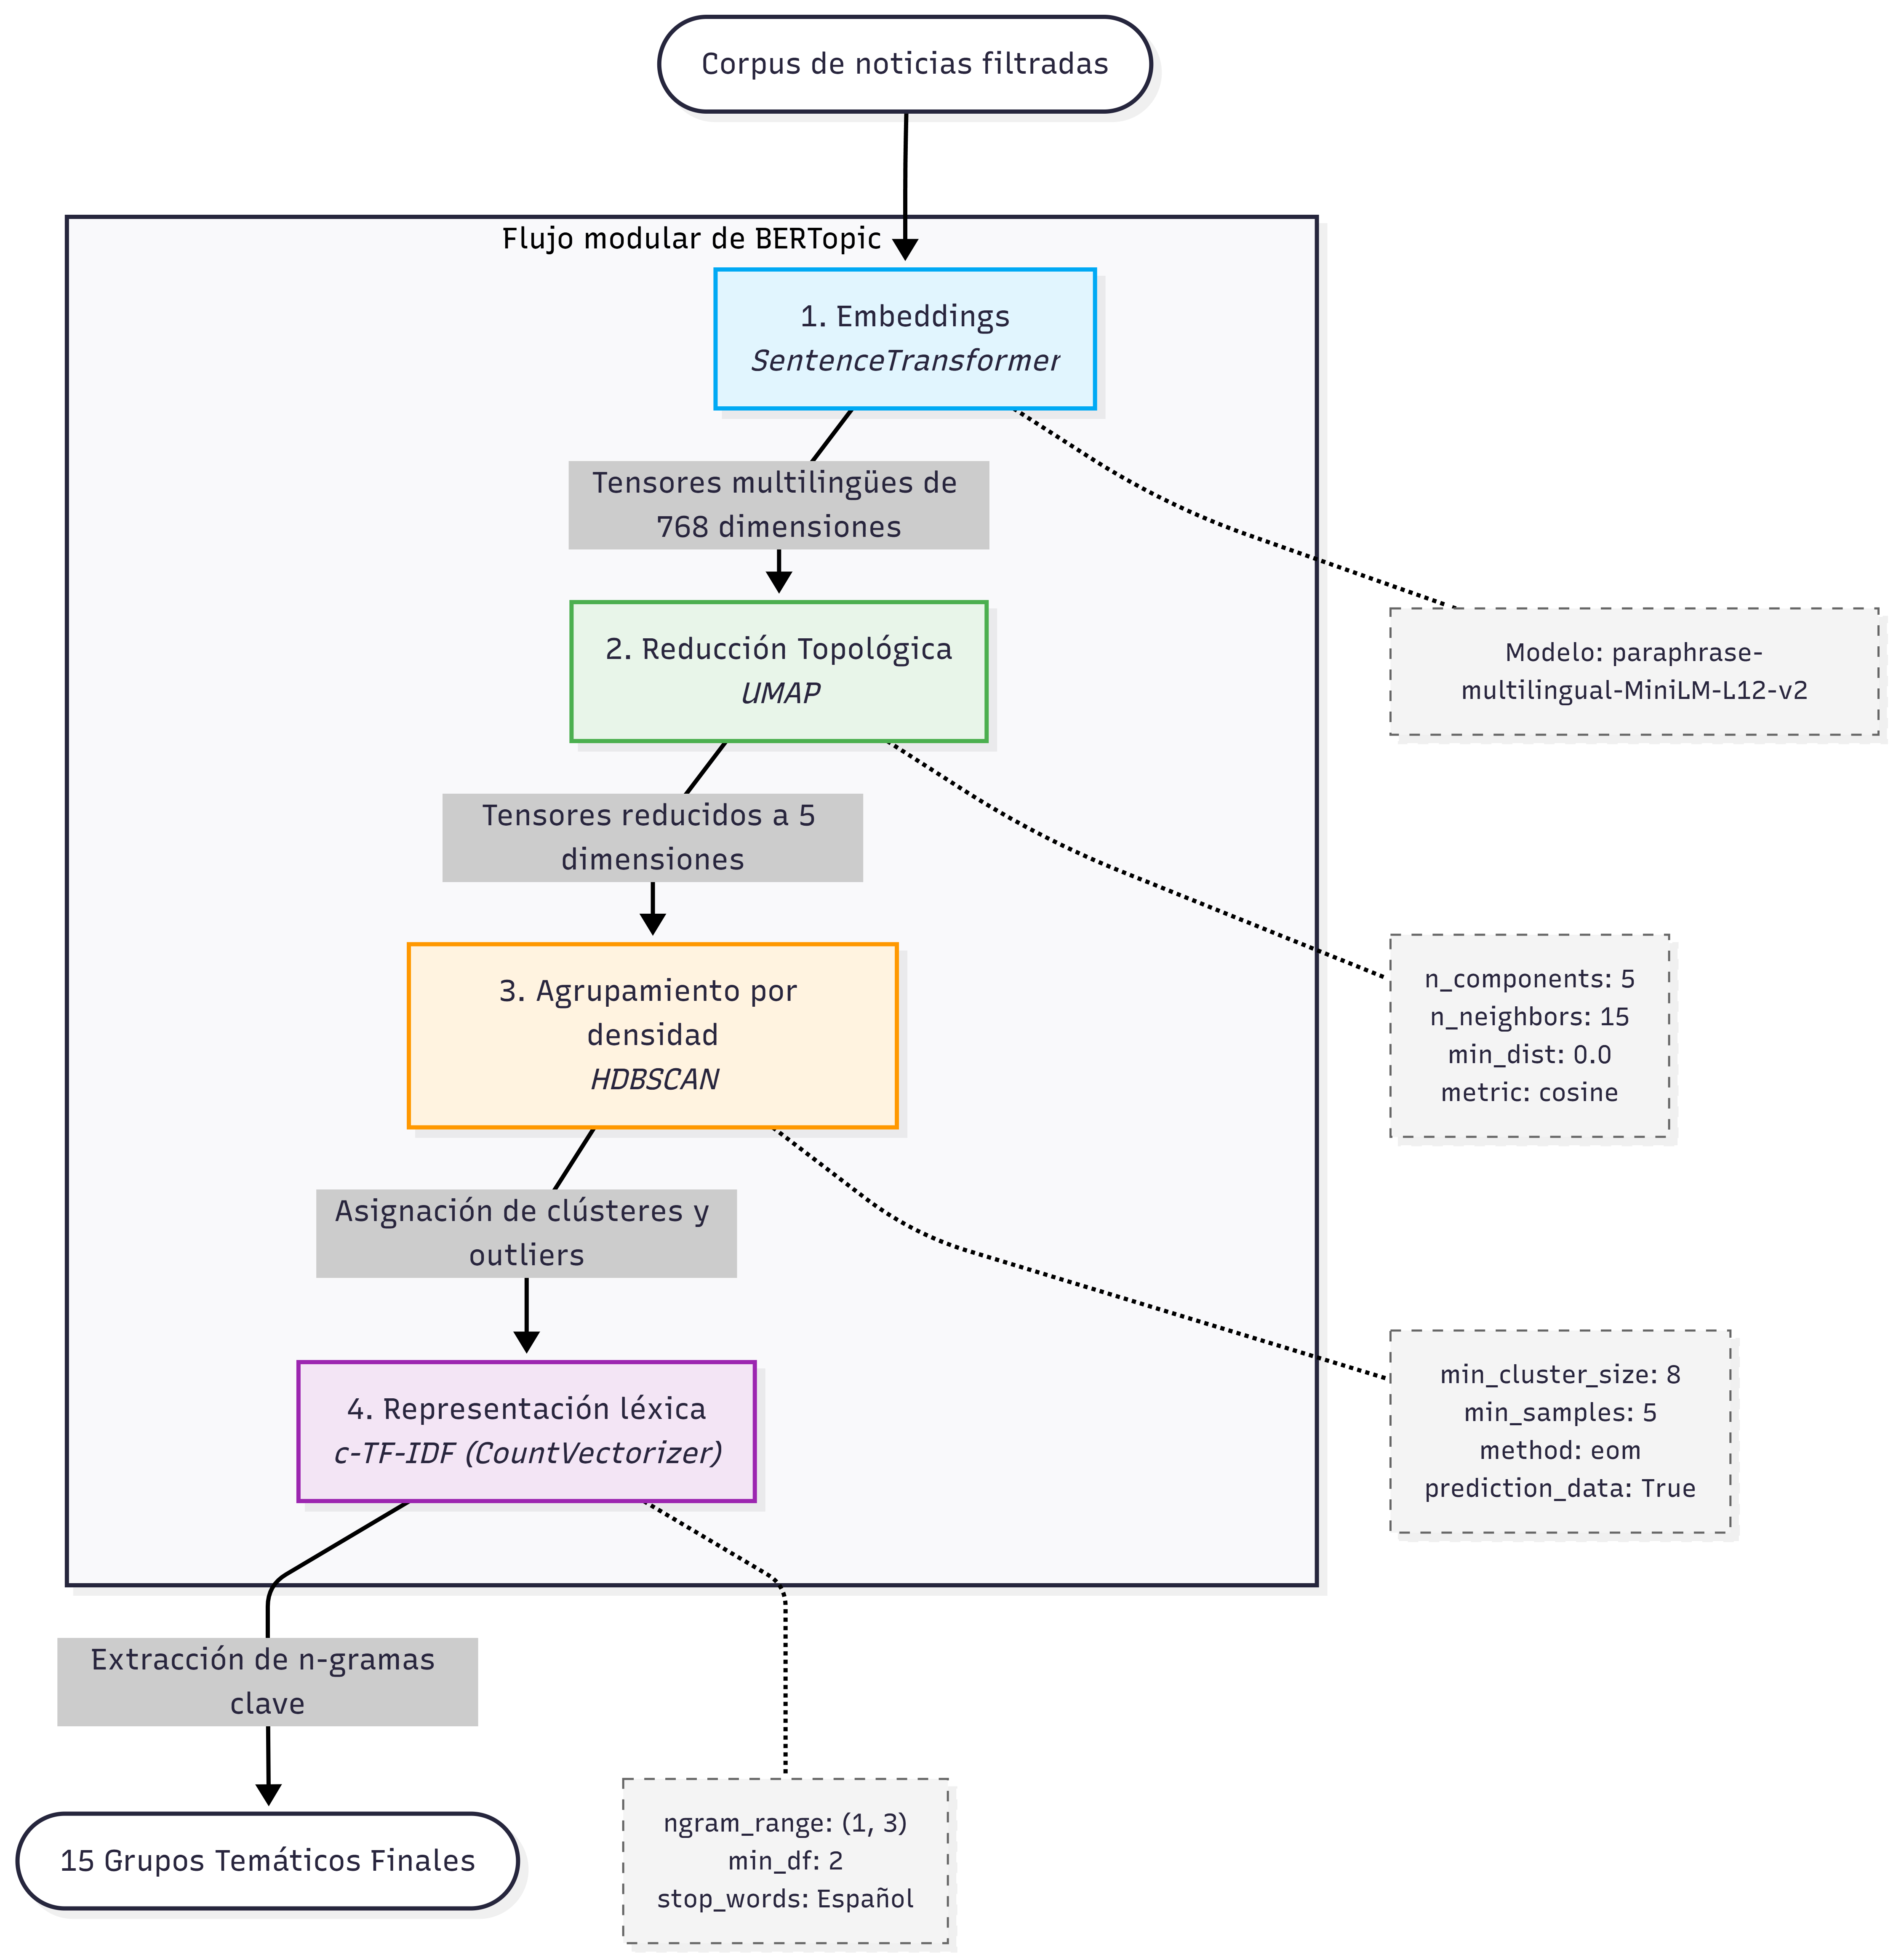
\includegraphics[width=\textwidth]{images/bertopicdiag.png}
    \caption{Arquitectura modular de BERTopic y su parametrización en TT II}
    \label{fig:bertopic_proceso}
\end{figure}

\subsubsection{UMAP}
\label{subsubsec:ea_umap}

UMAP (\textit{Uniform Manifold Approximation and Projection}) \cite{mcinnes2018umap}
proyecta los vectores de 768 dimensiones generados por BETO hacia un espacio de
5 dimensiones lo que resuelve la maldición de la dimensionalidad de K-Means.
A diferencia de PCA (que preserva únicamente varianza global lineal) y t-SNE
(que preserva solo estructura local y no escala a más de 50{,}000~puntos),
UMAP preserva simultáneamente la estructura topológica local y global de los
documentos semánticamente similares y que permanecen adyacentes en el espacio reducido.
Por otro lado mantiene separados a los documentos semánticamente distintos.

La configuración \texttt{metric='cosine'} es determinante pues los embeddings de texto
tienen magnitudes variables y la similitud semántica se mide por el ángulo entre
vectores (similitud coseno) no por su distancia euclidiana. Usar UMAP con métrica
coseno garantiza que la estructura topológica preservada sea semánticamente
significativa. El parámetro \texttt{min\_dist=0.0} fuerza a que los puntos dentro
de cada clúster se compriman máximamente lo que aumenta la densidad local y
la detección de fronteras por HDBSCAN.

\subsubsection{HDBSCAN}
\label{subsubsec:ea_hdbscan}

HDBSCAN \cite{campello2013hdbscan} (\textit{Hierarchical DBSCAN}) extiende DBSCAN
construyendo una jerarquía de clústeres en función de la densidad local de cada
punto sin requerir un $\varepsilon$ global. La selección de clústeres mediante el
método \textit{Excess of Mass} (EoM) identifica automáticamente las particiones
óptimas en la jerarquía generando clústeres de densidades heterogéneas. Los puntos
que no pertenecen a ningún clúster de densidad suficiente reciben la etiqueta de
ruido (\texttt{topic\_id = -1}).

Esta propiedad de detección de ruido es semánticamente valiosa en el dominio del
sistema pues las noticias \textit{outlier} (o sin coherencia temática con el corpus)
son exactamente las que el sistema debe tratar con mayor escrutinio en la
clasificación semántica elevando su umbral de exigencia de BETO de 0.50 a 0.65.
El código de \texttt{bertopic\_clustering.py} documenta que los datos reales presentaron 
nicialmente \textbf{81.4\% de outliers} resueltos mediante
una reducción multi-etapa de tres estrategias progresivas.

\begin{figure}[H]
    \centering
    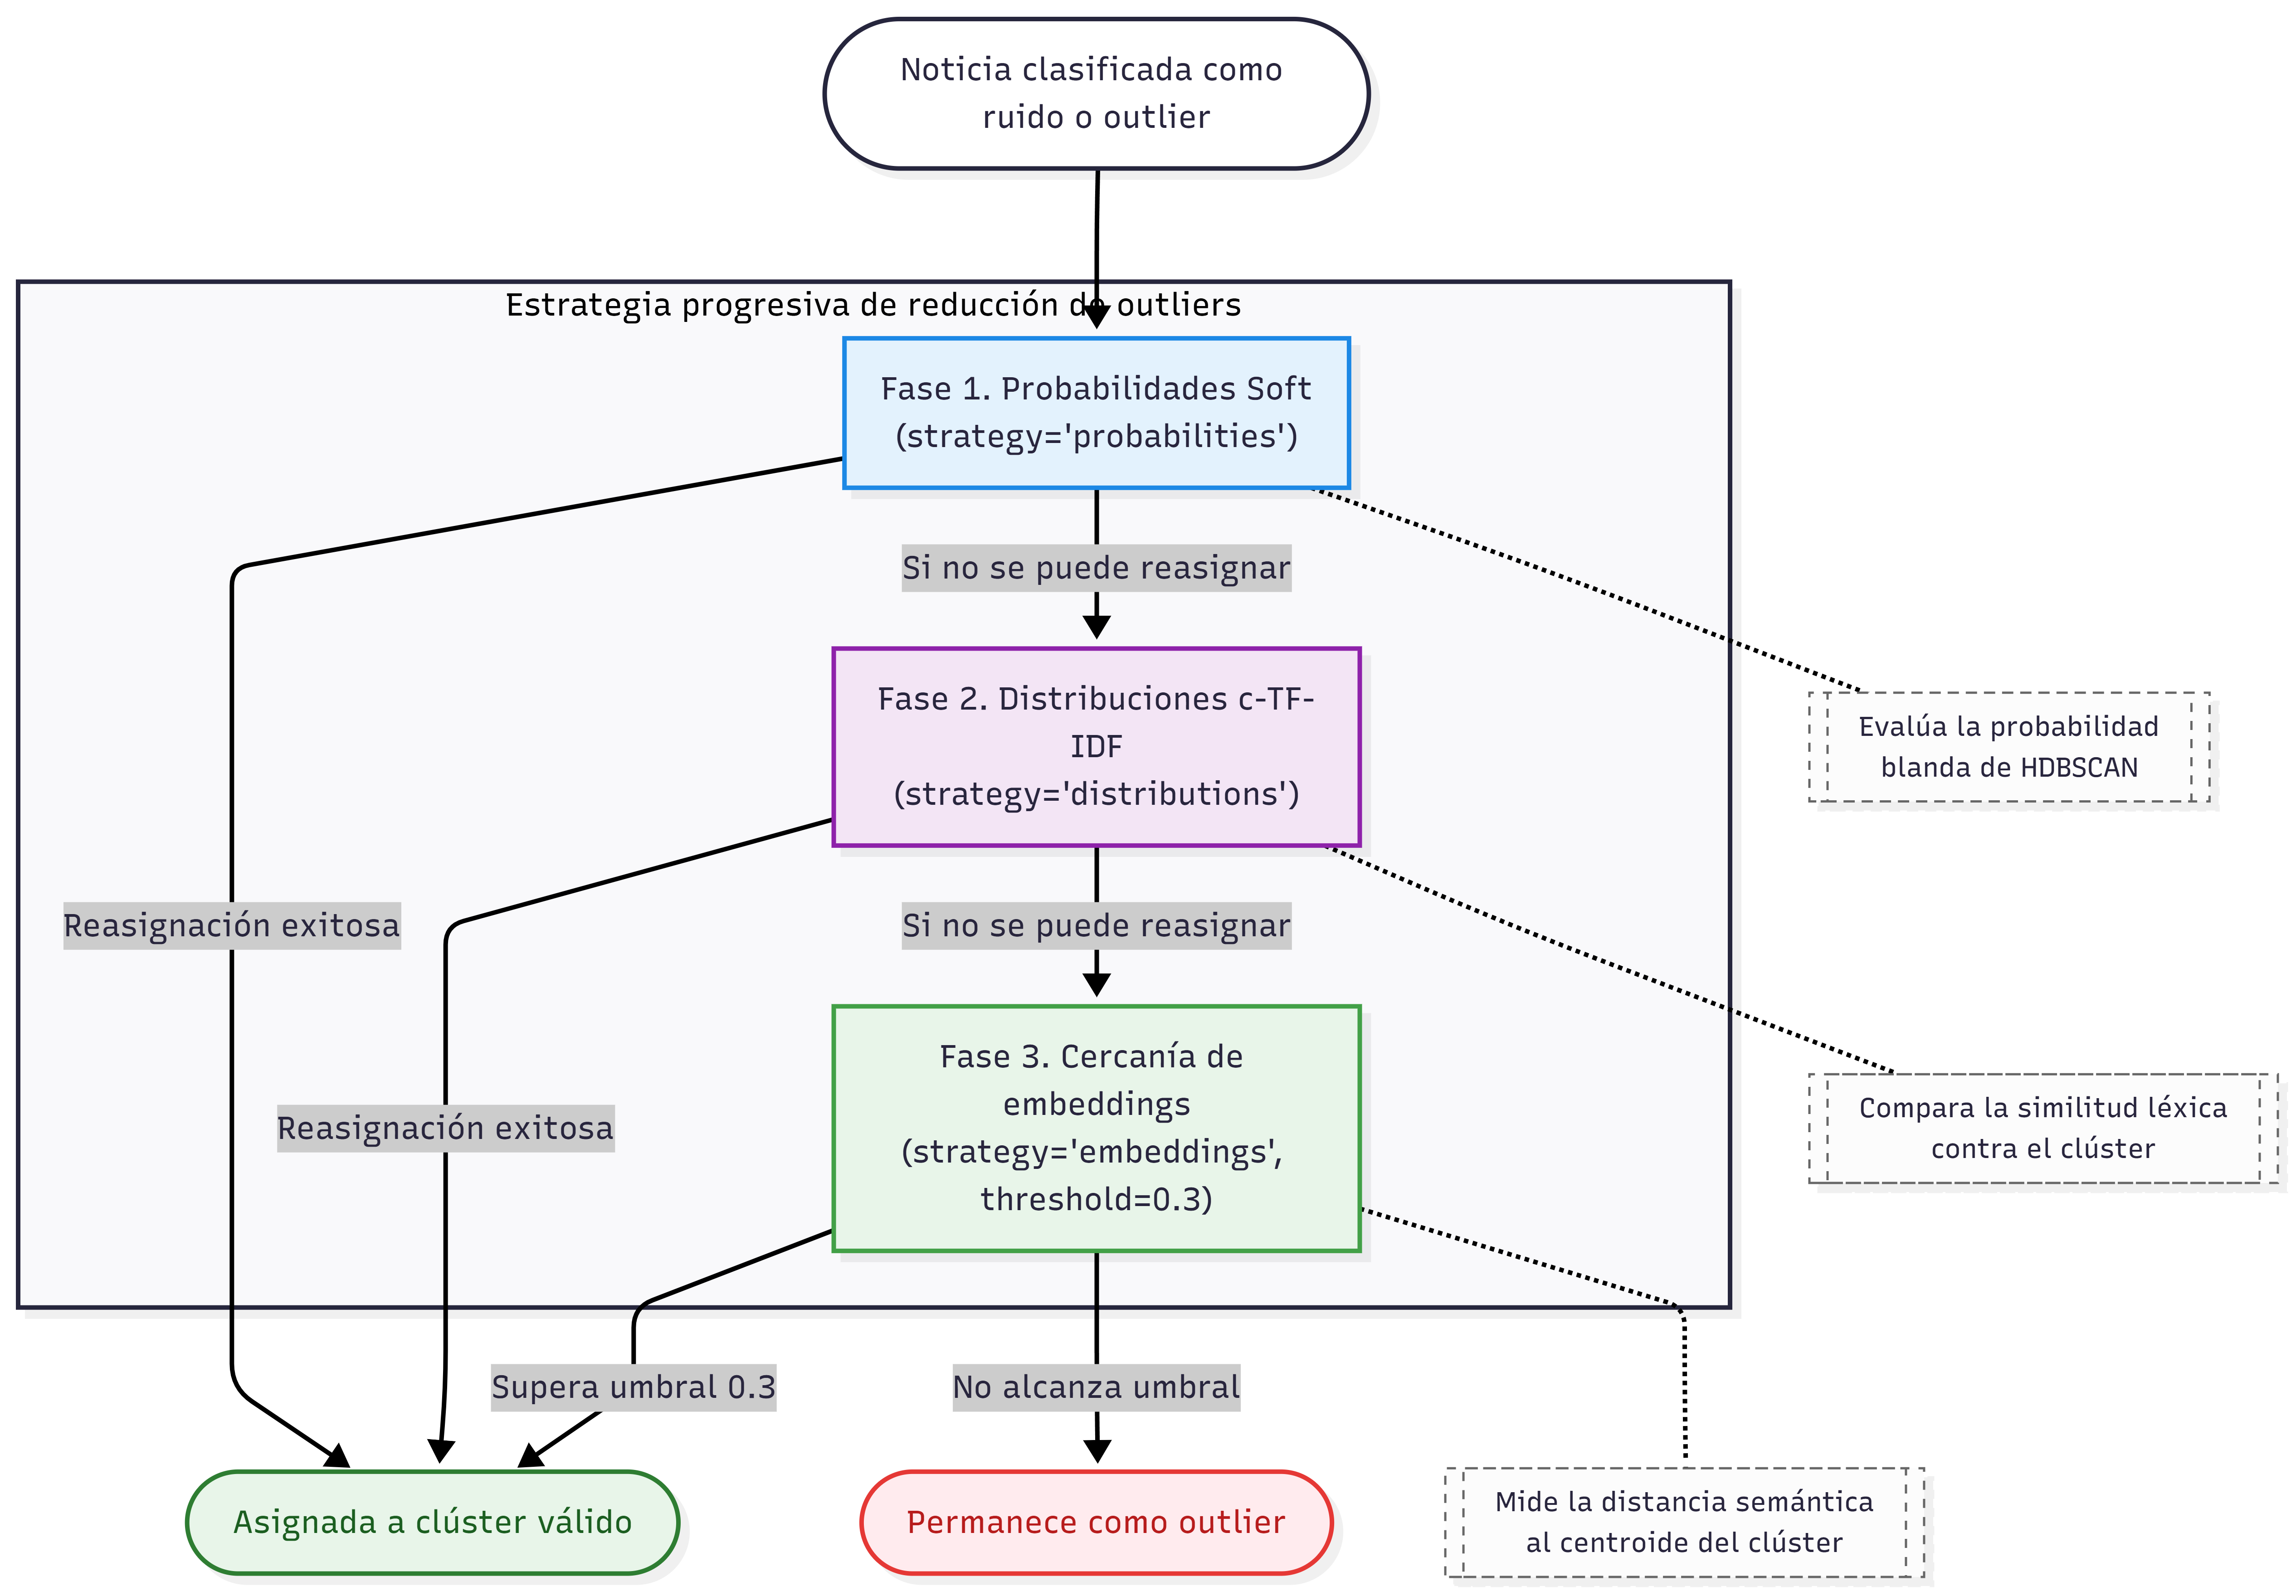
\includegraphics[width=\textwidth]{images/outliers.png}
    \caption{Reducción de outliers en BERTopic}
    \label{fig:outliers}
\end{figure}

\subsubsection{c-TF-IDF}
\label{subsubsec:ea_ctfidf}

La representación de cada tópico se obtiene mediante \textit{Class-based TF-IDF}
(c-TF-IDF) \cite{grootendorst2022bertopic} aqui el algoritmo concatena todos los
documentos de un mismo clúster en un ``mega documento de clase'' y aplica TF-IDF
comparando cada clase contra el corpus completo. Esto identifica los términos
que son frecuentes dentro del clúster pero infrecuentes en el resto del corpus,
lo que genera representaciones léxicas interpretables que caracterizan semánticamente
cada tópico.

El vectorizador configurado con \texttt{ngram\_range=(1, 3)} permite que las
representaciones incluyan frases de hasta tres palabras lo que captura expresiones
compuestas de alta especificidad para el dominio (por ejemplo
\textit{``víctima de feminicidio''}, \textit{``hijos resguardados DIF''}).
La representación final por tópico mediante \texttt{KeyBERTInspired} refina
adicionalmente los términos seleccionados usando similitud coseno entre el embedding
del n-grama y el embedding promedio de los documentos del clúster lo que garantiza
que las palabras clave seleccionadas sean semánticamente representativas y no solo
estadísticamente frecuentes.

\subsection{Evolución comparativa de TT I a TT II de Léxico a Semántica}
\label{subsec:ea_evolucion_clustering}

La Tabla~\ref{tab:comparativa_clustering} sintetiza la evaluación de los tres
algoritmos de agrupamiento en función de los criterios operativos del sistema.

\vspace{0.5cm}
\begin{table}[htbp]
\centering
\caption{Comparativa de algoritmos de agrupamiento semántico para corpus periodístico}
\label{tab:comparativa_clustering}
\begin{tabular}{|p{2.8cm}|p{2.8cm}|p{2.8cm}|p{3.0cm}|}
\hline
\textbf{Criterio} &
\textbf{K-Means} \newline (TT1) &
\textbf{DBSCAN} &
\textbf{BERTopic} \newline (UMAP+HDBSCAN, TT2) \\
\hline
\textbf{Manejo de ruido} &
Ninguno (todos los puntos asignados a un clúster) &
Sí (puntos en baja densidad = ruido) &
Sí (HDBSCAN con reducción multi-etapa 81.4\%→55\%) \\
\hline
\textbf{Escalabilidad} &
Alta ($O(n \cdot k \cdot i)$) &
Media ($O(n^2)$ sin índice espacial) &
Alta (UMAP+HDBSCAN: $O(n \log n)$ aproximado) \\
\hline
\textbf{Interpretación de tópicos} &
Baja (centroides en espacio de alta dimensión sin interpretabilidad) &
Ninguna (solo densidad geométrica) &
Alta (c-TF-IDF genera top n-grams interpretables por tópico) \\
\hline
\textbf{Dependencia de parámetros} &
Crítica ($k$ fijo requerido) &
Alta ($\varepsilon$ global uniforme) &
Baja (\texttt{min\_cluster\_size=8} adaptativo; $k$ automático) \\
\hline
\textbf{Alta dimensionalidad} &
Muy baja (maldición de la dimensionalidad) &
Baja (distancias euclidianas en alta dimensión) &
Alta (UMAP reduce a 5D preservando topología) \\
\hline
\textbf{Resultado en TT1/TT2} &
\textit{Descartado en TT2} (clústeres no coherentes) &
\textit{Evaluado} (inadecuado por $\varepsilon$ global) &
\textbf{Seleccionado} (OE-4, P4) \\
\hline
\end{tabular}
\end{table}
\vspace{0.4cm}

La diferencia más significativa entre TT I y el TT II en materia de
agrupamiento no es algorítmica sino epistemológica pues en TT I el agrupamiento
K-Means operaba sobre \textbf{vectores TF-IDF léxicos} donde dos documentos son
similares si comparten los mismos tokens literales. En el TT II BERTopic opera sobre
\textbf{embeddings semánticos de BETO} donde dos documentos son similares si
expresan el mismo \textit{significado} independientemente del vocabulario utilizado.

Esta distinción tiene una consecuencia operativa directa en TT II como que noticias
publicadas por La Jornada, El Universal y Milenio sobre el \textit{mismo caso
criminal} de feminicidio aunque redactadas con vocabularios completamente
distintos, diferentes tiempos verbales y enfoques editoriales estarán en el mismo
clúster BERTopic pues sus embeddings BETO convergen en la misma región del espacio
semántico. En el TT I estas tres noticias podían dispersarse en tres clústeres K-Means
distintos por la mínima varianza léxica entre medios.


\section{Conclusión del capítulo}
\label{sec:ea_conclusion}


El análisis del estado del arte desarrollado revela que ninguna de las tecnologías
examinadas de forma aislada es suficiente para resolver el problema social planteado.
La recolección mediante RSS provee eficiencia pero no comprensión, TF-IDF provee velocidad
pero no contexto, K-Means provee estructura pero no semántica, BETO provee comprensión
pero puede alucinar sin reglas simbólicas.

La innovación fundamental de este Trabajo Terminal no radica en la invención de ningún algoritmo
nuevo sino en la orquestación de tecnologías y estrategias que se fueron adaptando a lo largo del
desarrollo del sistema (RSS unida a la infraestructura de \texttt{StealthSession},
deduplicación en cascada, persistencia relacional en PostgreSQL, el modelo Transformer monolingüe
\textbf{BETO Fine-Tuned}, el entorno de modelado de tópicos \texttt{BERTopic},
el algoritmo híbrido de \textbf{clasificacion escalonada} y el módulo de \textbf{investigación profunda})
en un flujo de datos coherente y específicamente calibrado para un dominio social complejo.

Cada decisión tecnológica documentada en este capítulo puede trazarse directamente a una necesidad
social concreta.

\begin{itemize}
    \item La elección de RSS sobre scraping estático garantiza cobertura sostenida sin saturar los
          servidores de medios independientes con recursos limitados, \texttt{StealthSession}
          extiende esta cobertura al 35\% de fuentes sin feed RSS mediante emulación de
          fingerprint TLS.
    \item La deduplicación en cascada (MD5 → Jaccard → SimHash → coseno TF-IDF) garantiza que un
          mismo caso cubierto por múltiples medios con vocabulario diferente no
          genere alertas redundantes.
    \item La migración a PostgreSQL con FTS garantiza que los trabajadores sociales puedan
          consultar el sistema en tiempo real con latencia $O(\log n)$ sin esperar escaneos
          lineales de CSV.
    \item La elección de BETO sobre mBERT garantiza que el sistema comprende el español coloquial
          y periodístico mexicano con la misma precisión que el español académico.
    \item La clasificación escalonada garantiza que el sistema nunca clasificará a un menor agresor
          como víctima indirecta ni descartará un caso real de orfandad por la ambigüedad
          redaccional de un periodista local.
    \item La investigación profunda garantiza que los analistas dispongan de fichas de caso
          estructuradas con ubicación, número de NNA afectados, situación actual e institución
          competente para cada caso que merezca intervención, sin depender de búsquedas
          manuales en portales de noticias.
\end{itemize}

En suma este trabajo terminal presenta un ecosistema tecnológico diseñado para
garantizar que ningún caso de niña, niño o adolescente que quedó en orfandad por
feminicidio sea invisible para las instituciones del Estado que tienen la obligación legal
de protegerlo.